% Appendices do not count toward the 7-page limit.
% Good homes for: full CPTs, derivations, extra configurations, code pointers.

\section{M-Step Under a Dirichlet Prior}
\label{app:em}
For one CPT row with parent configuration $u$, the M-step maximizes the
expected log-likelihood plus the log-prior,
\begin{equation*}
  \sum_x \bigl(\hat N(x,u) + \alpha\bigr) \log \theta_{x \mid u}
  \quad\text{subject to}\quad \sum_x \theta_{x \mid u} = 1,
\end{equation*}
where $\alpha \log \theta_{x \mid u}$ is the log-density of a symmetric
Dirichlet$(\alpha + 1)$ prior, up to a constant. Adding a Lagrange multiplier
$\lambda$ and setting the derivative to zero gives
$\theta_{x \mid u} = (\hat N(x,u) + \alpha)/\lambda$; the constraint fixes
$\lambda = \sum_{x'} \hat N(x',u) + K_X \alpha$, which is the update in
\cref{sec:em}. Rows are independent, so each is solved separately.

% Optional: P(gas | Event) table (3 states x 3 gases x 3 bins) from
% notebooks/phase3b/eval.ipynb, section 6, if it is not in Sec. 4.

\section{Network Variants}
\label{app:networks}
We built the model in stages, each adding one feature to the network. The
baseline is the simplest model: each gas depends only on the hour,
$P(G_j \mid H)$, and the sensors are ignored. Phase~1 adds the sensors for a
single gas, CO. Phase~2 adds NO$_x$ and NO$_2$ and the cross-sensitivity edges
from \cref{app:cross}; it is the ablation for Q2. Phase~3a \todo{one line: what
3a adds}. Phase~3b, the final model (\cref{fig:network}), replaces
hour~$\to$~gas with the latent emission regime (\cref{sec:latent}).

\begin{figure}[p]
  \centering
  \begin{subfigure}[t]{0.48\linewidth}
    \centering
    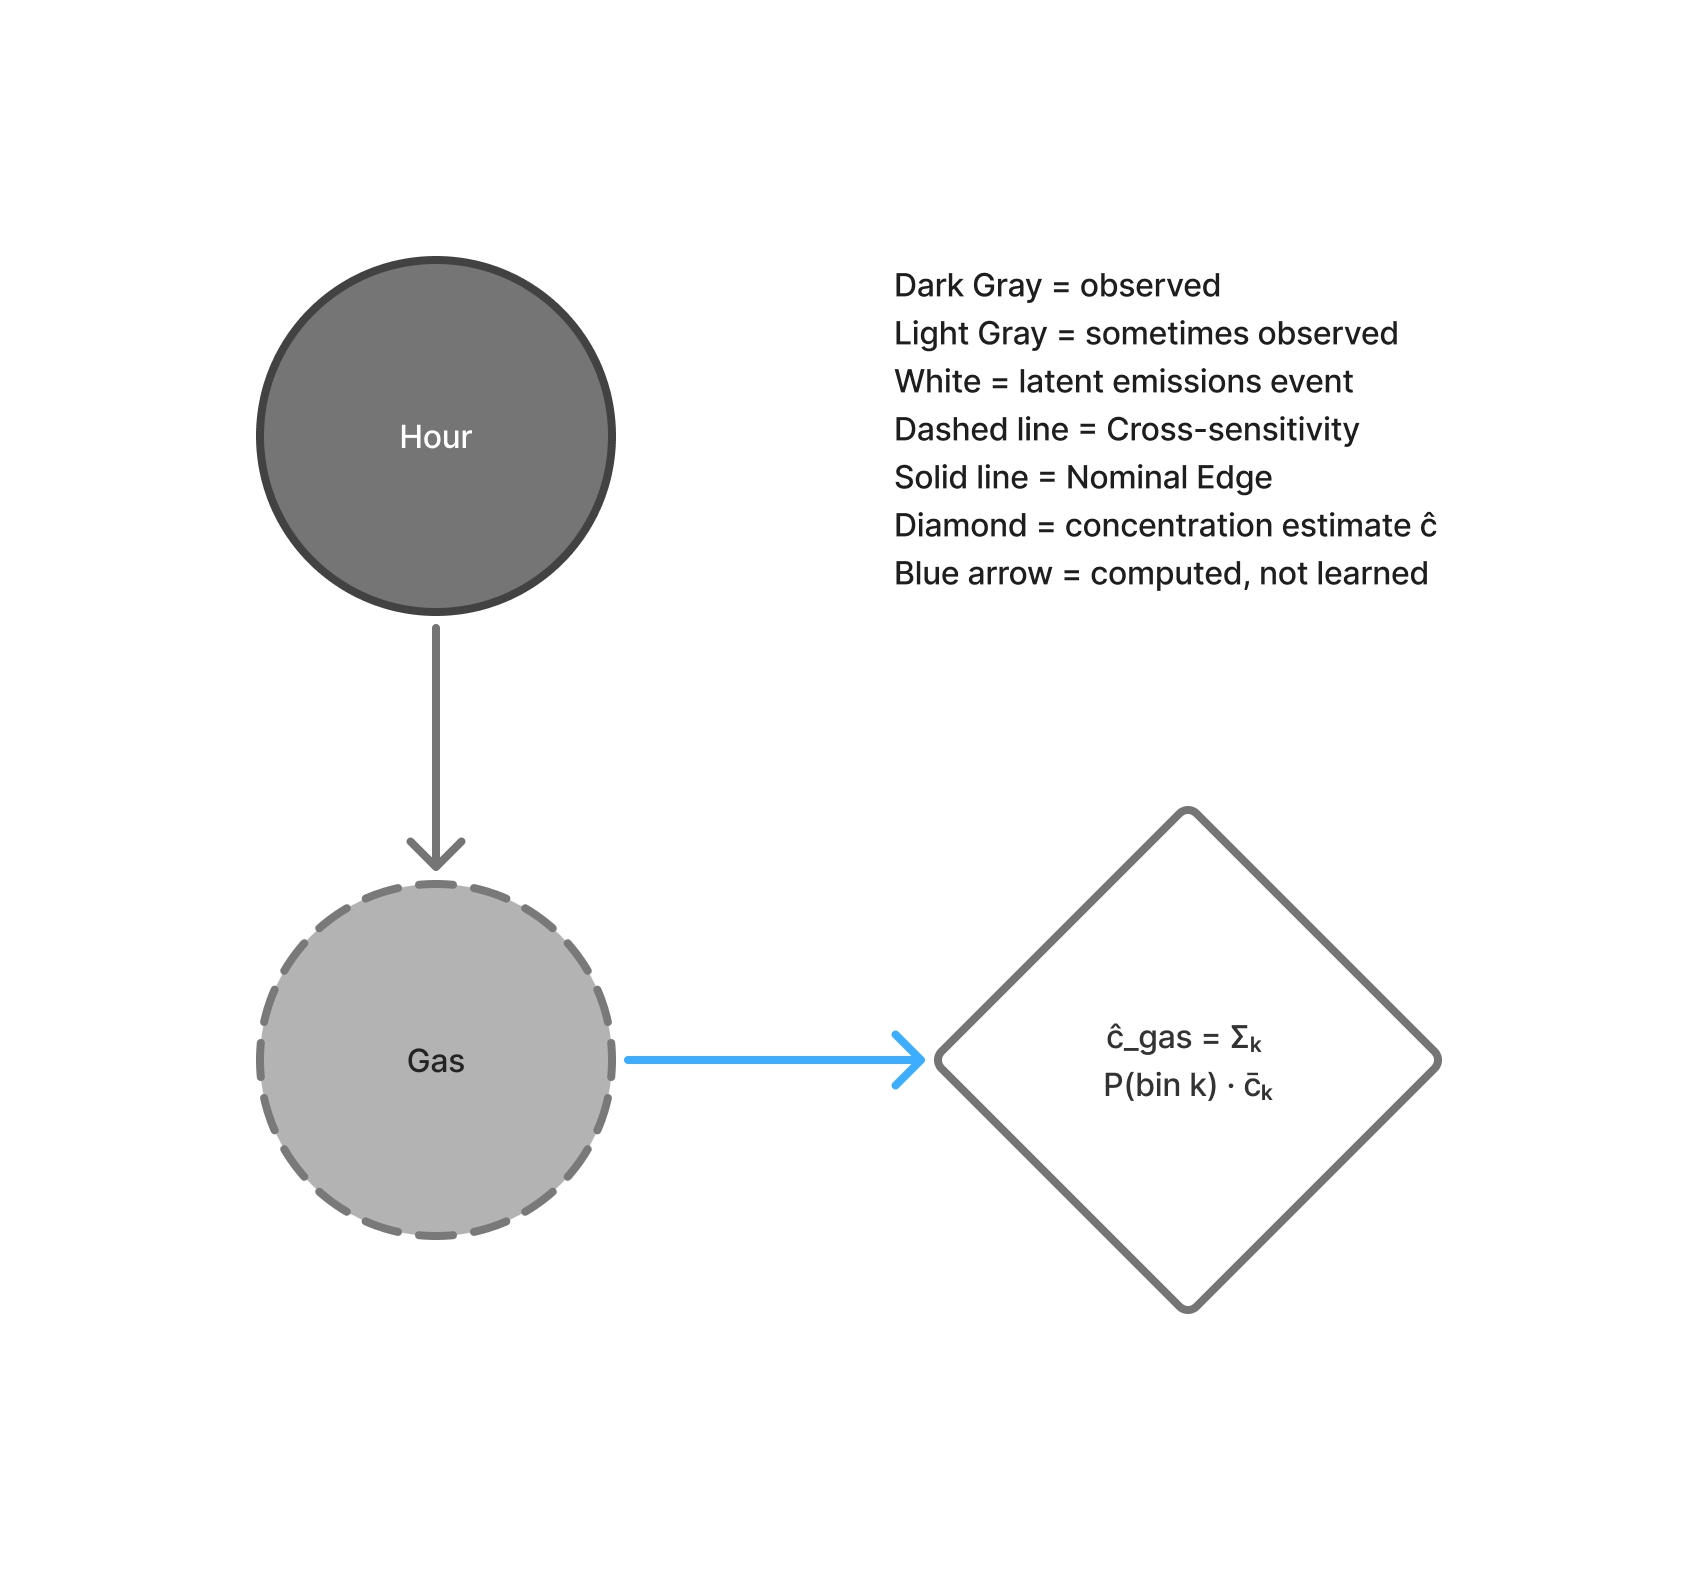
\includegraphics[width=\linewidth,height=0.25\textheight,keepaspectratio]{phase-0}
    \caption{Hour-only baseline.}
    \label{fig:net-baseline}
  \end{subfigure}\hfill
  \begin{subfigure}[t]{0.48\linewidth}
    \centering
    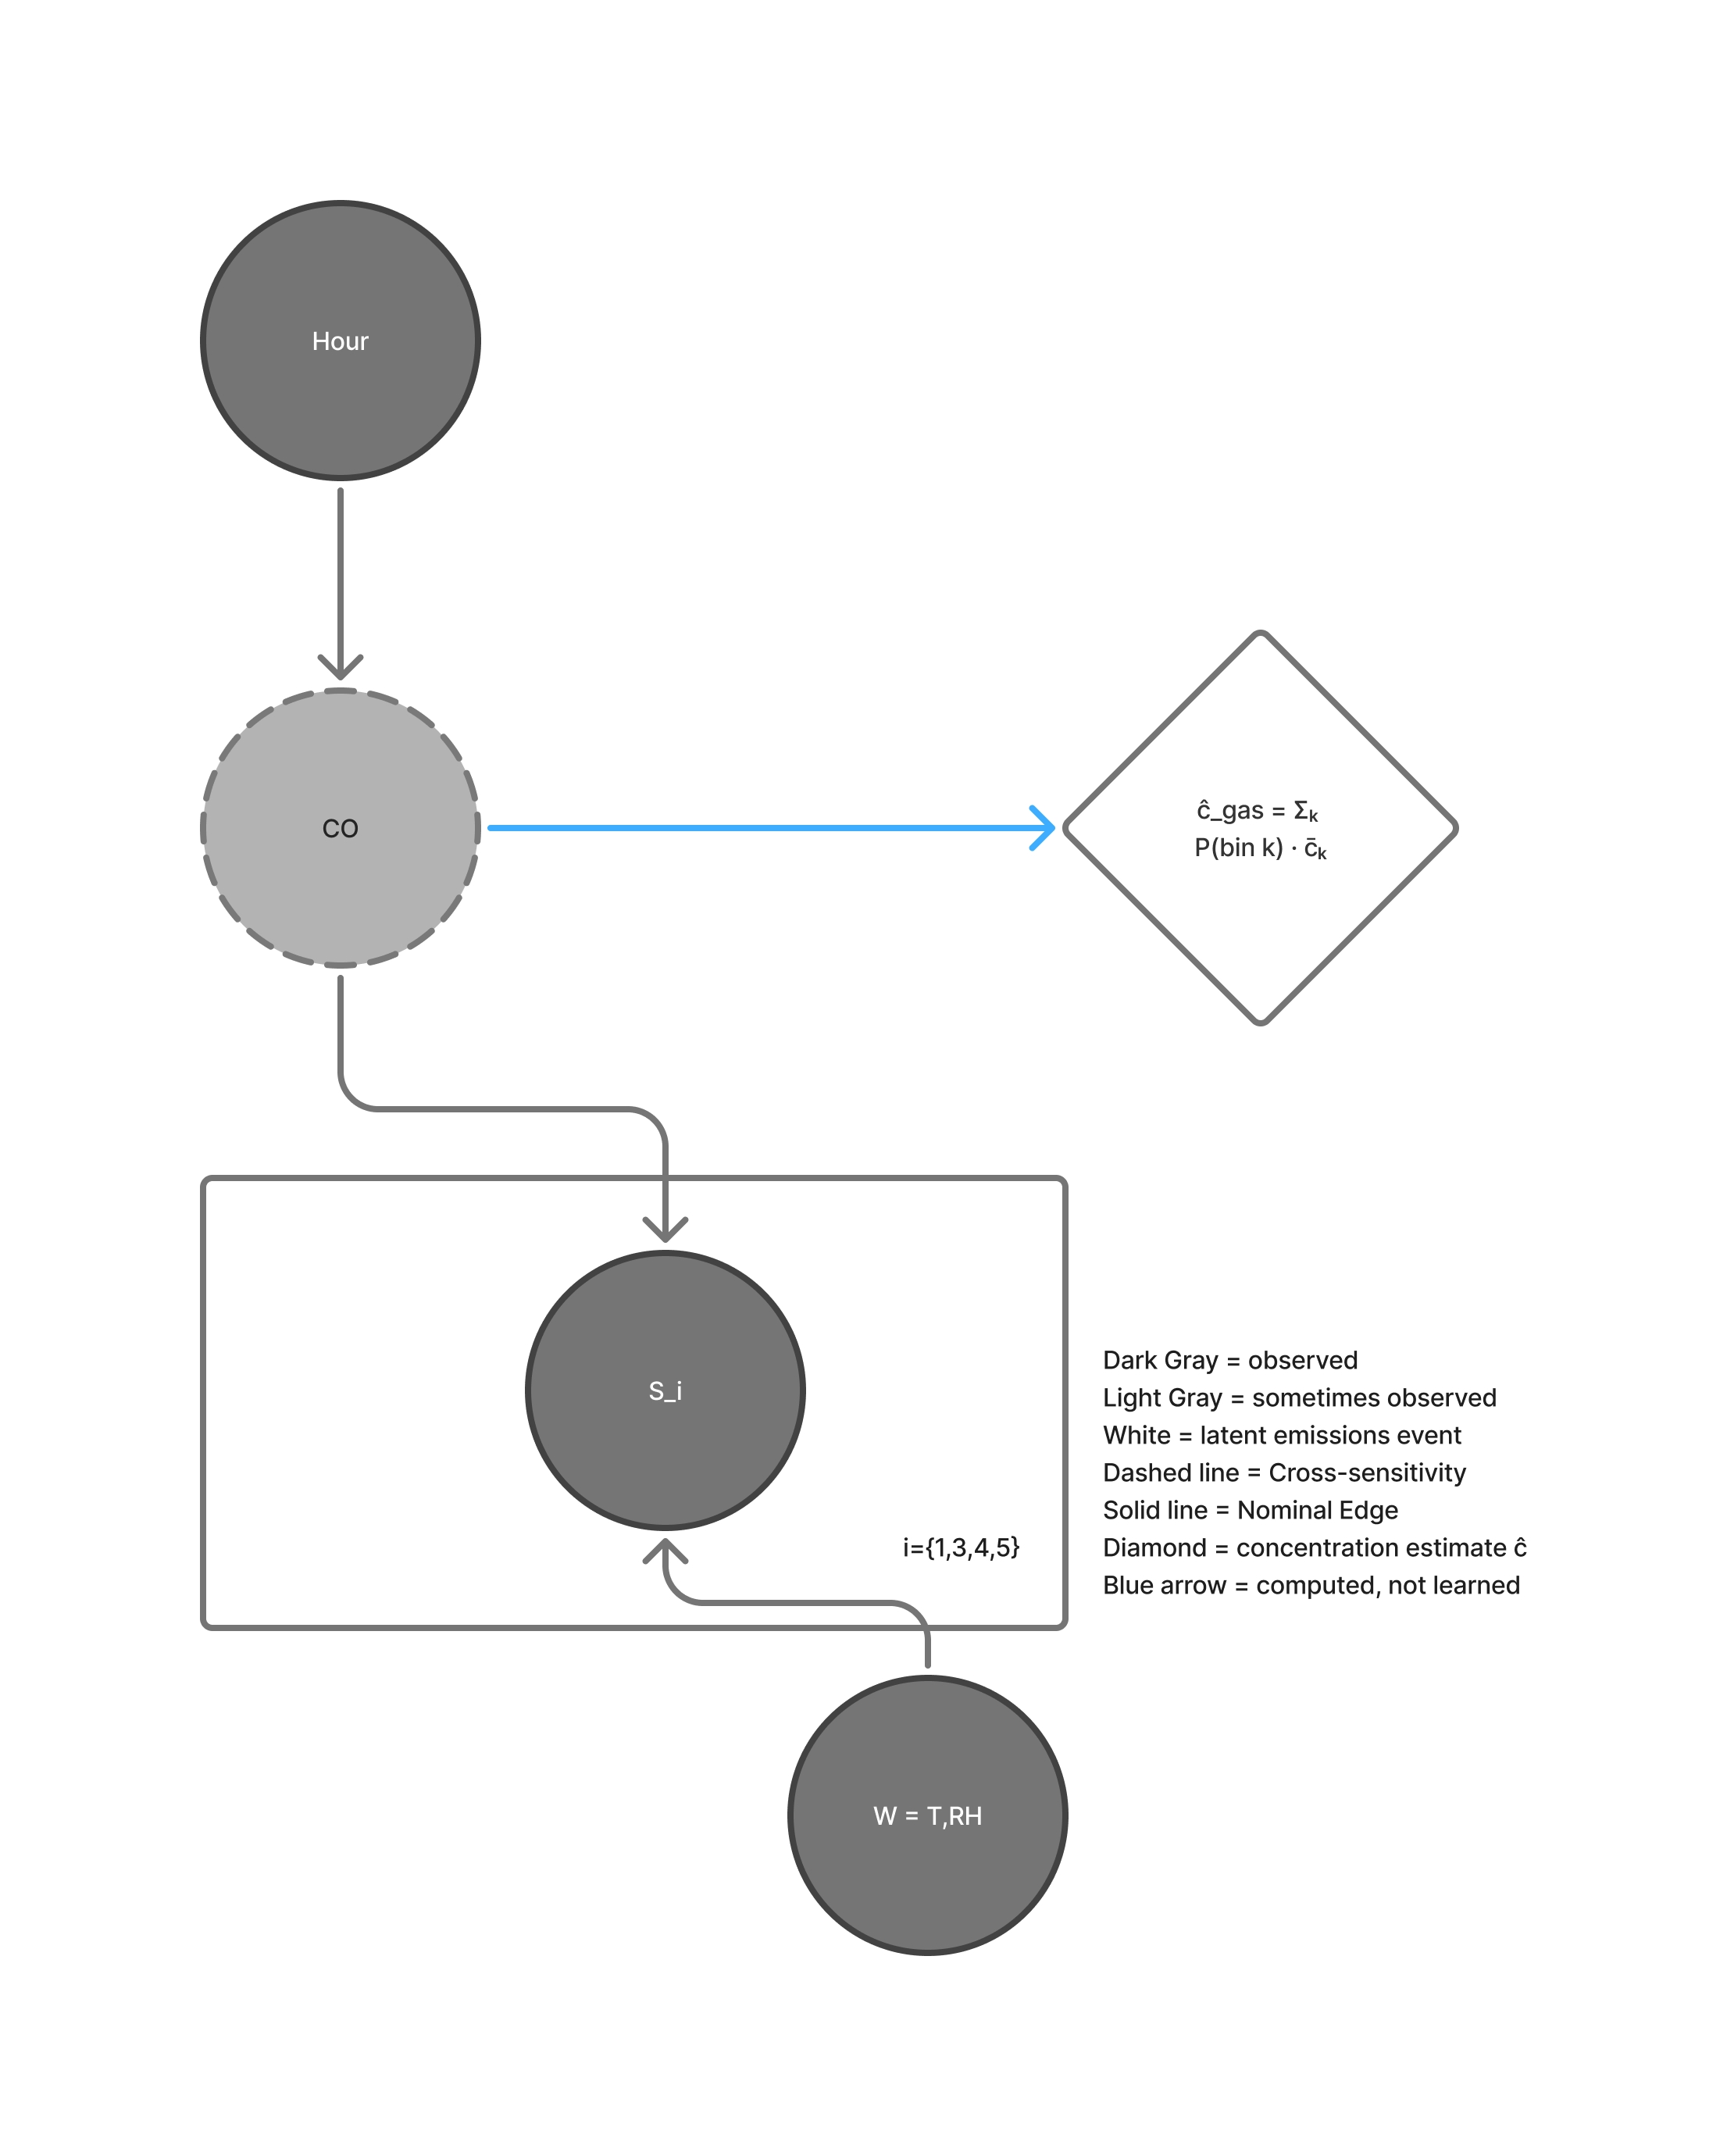
\includegraphics[width=\linewidth,height=0.25\textheight,keepaspectratio]{phase-1}
    \caption{Phase~1: CO only.}
    \label{fig:net-phase1}
  \end{subfigure}

  \vspace{0.8em}
  \begin{subfigure}[t]{0.48\linewidth}
    \centering
    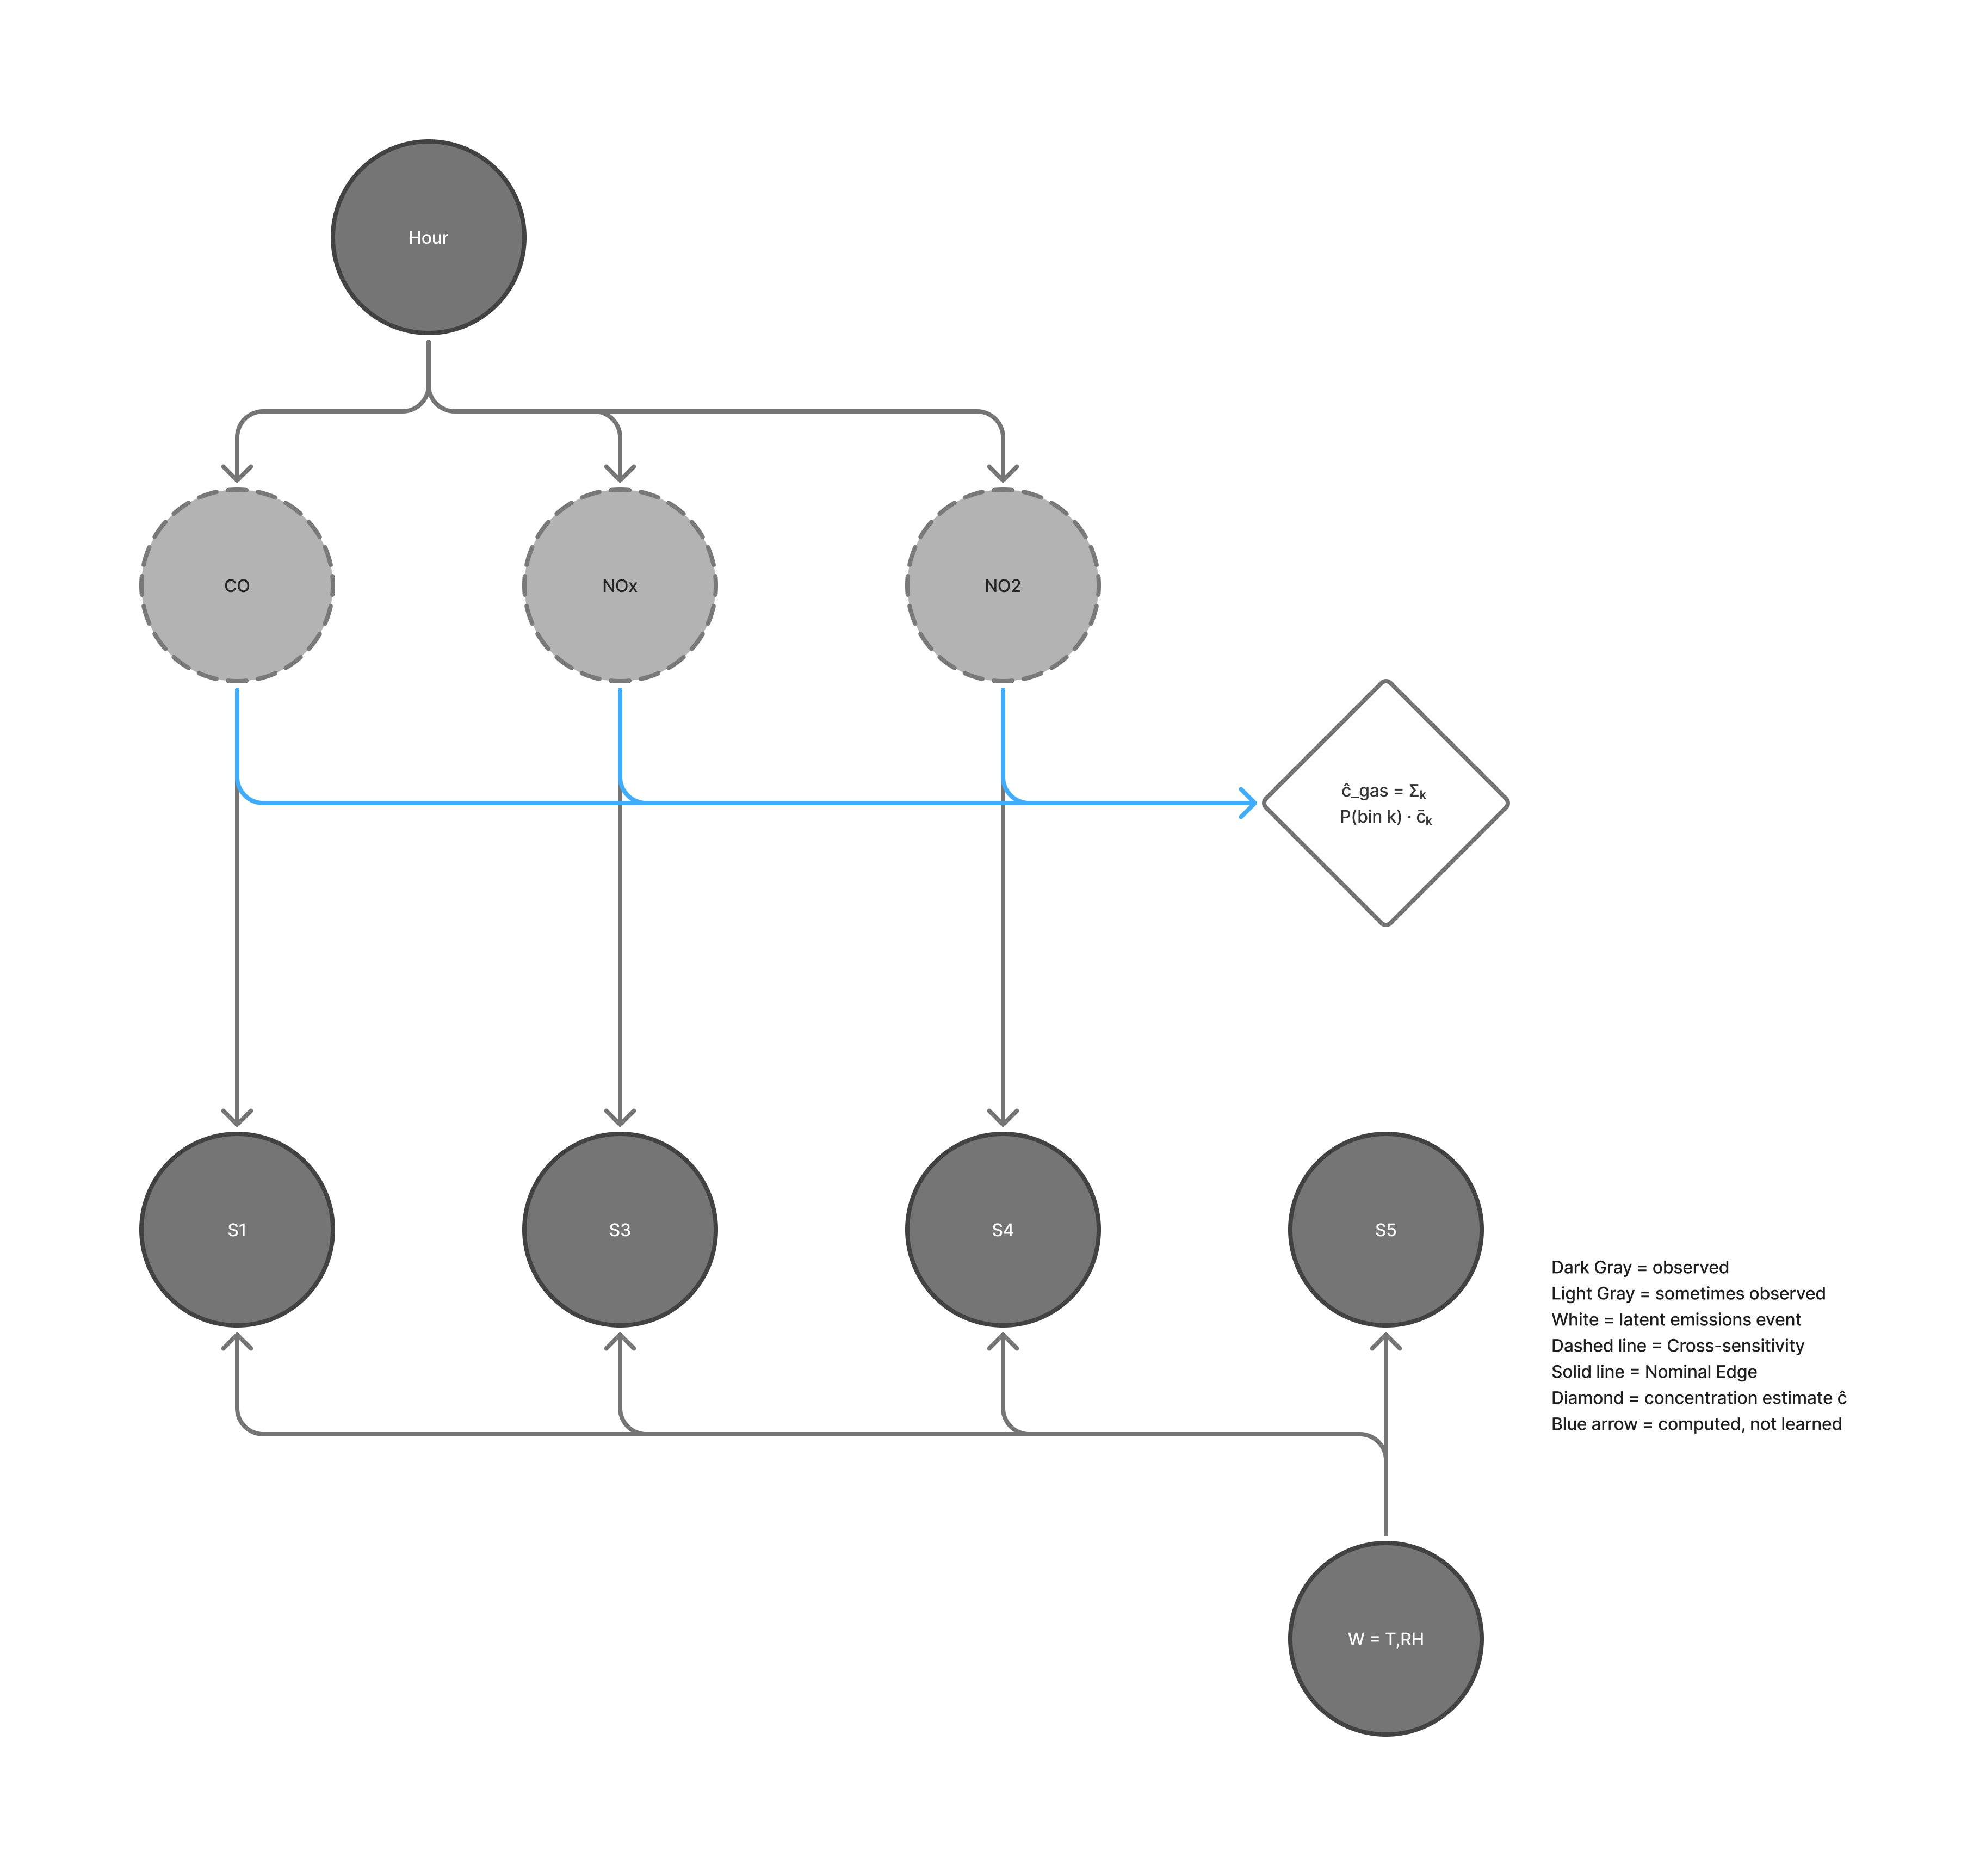
\includegraphics[width=\linewidth,height=0.25\textheight,keepaspectratio]{phase-2}
    \caption{Phase~2: three gases, cross-sensitivities.}
    \label{fig:net-phase2}
  \end{subfigure}\hfill
  \begin{subfigure}[t]{0.48\linewidth}
    \centering
    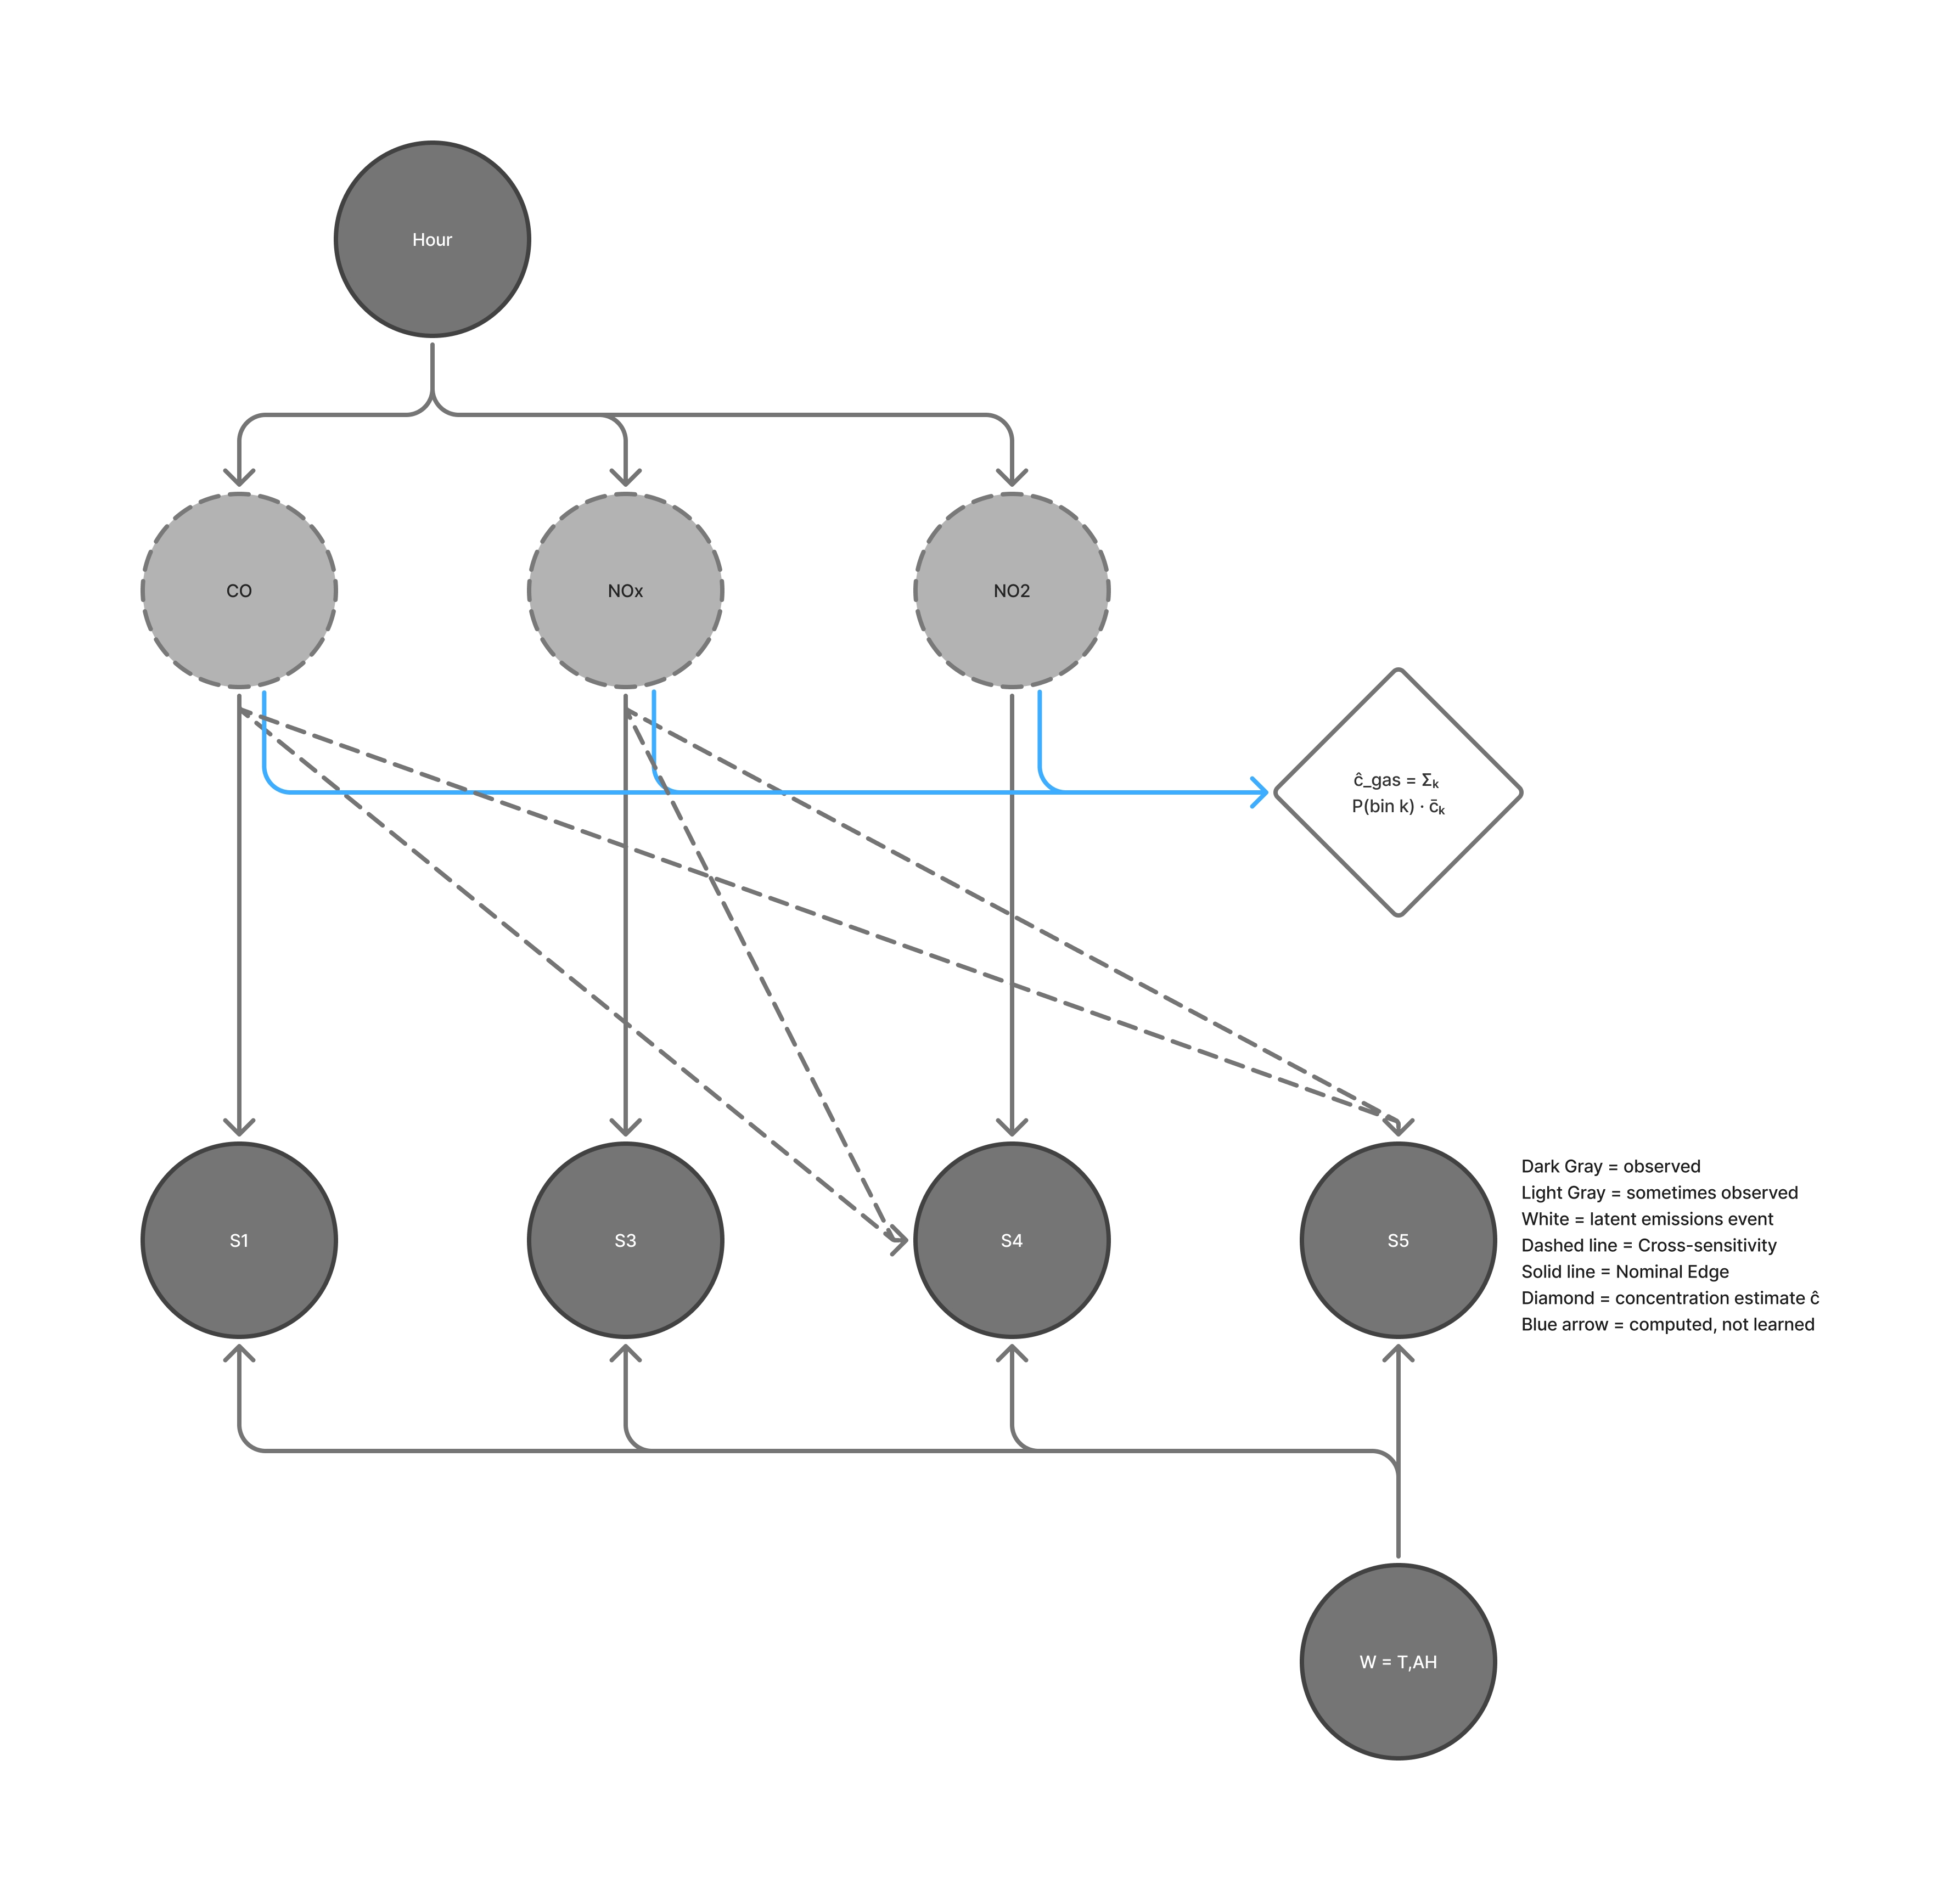
\includegraphics[width=\linewidth,height=0.25\textheight,keepaspectratio]{phase-3a}
    \caption{Phase~3a: \todo{short label}.}
    \label{fig:net-phase3a}
  \end{subfigure}

  \vspace{0.8em}
  \begin{subfigure}[t]{0.48\linewidth}
    \centering
    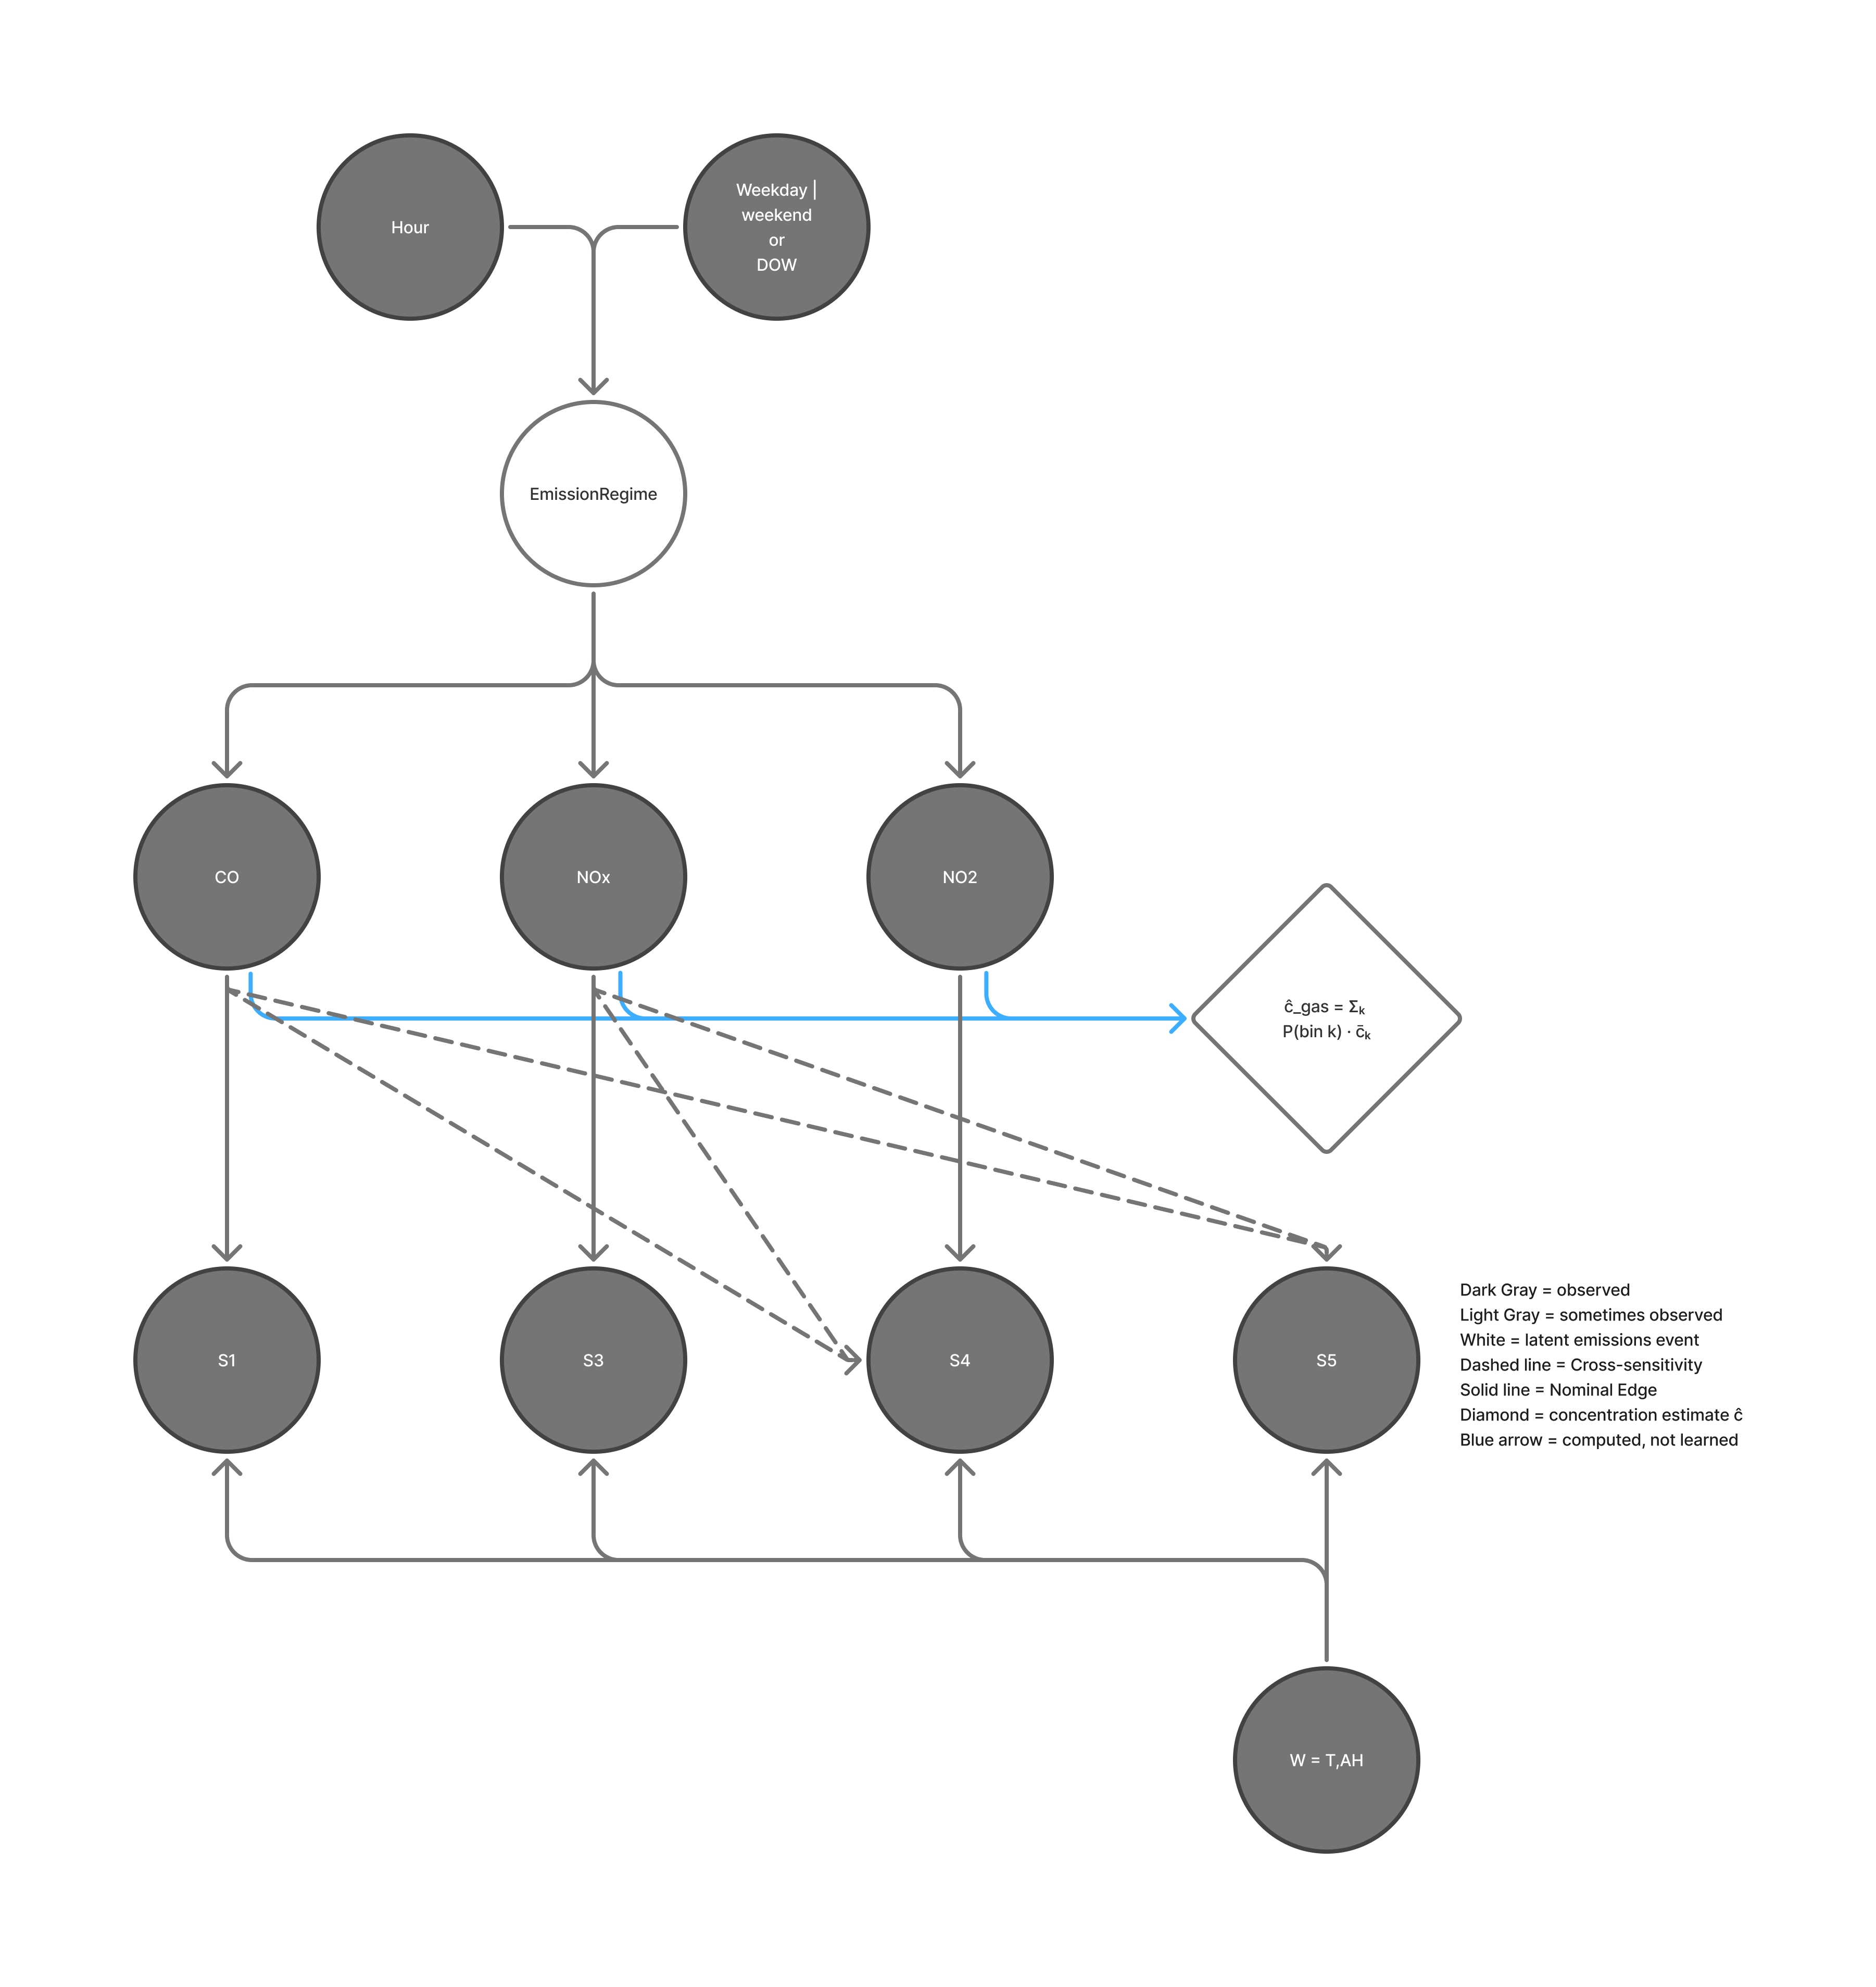
\includegraphics[width=\linewidth,height=0.25\textheight,keepaspectratio]{phase-3b}
    \caption{Phase~3b: latent emission regime (final; also \cref{fig:network}).}
    \label{fig:net-phase3b}
  \end{subfigure}
  \caption{Network for each phase, from the hour-only baseline to the final model.}
  \label{fig:net-variants}
\end{figure}

\section{Missing Data}
\label{app:missing}

\begin{figure}[h]
  \centering
  \begin{subfigure}[t]{0.48\linewidth}
    \centering
    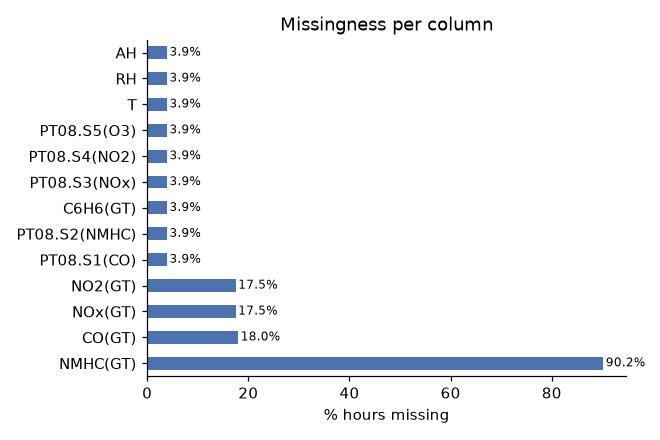
\includegraphics[width=\linewidth]{muska/missingness}
    \caption{Share of hours missing, per column.}
    \label{fig:missing-col}
  \end{subfigure}\hfill
  \begin{subfigure}[t]{0.48\linewidth}
    \centering
    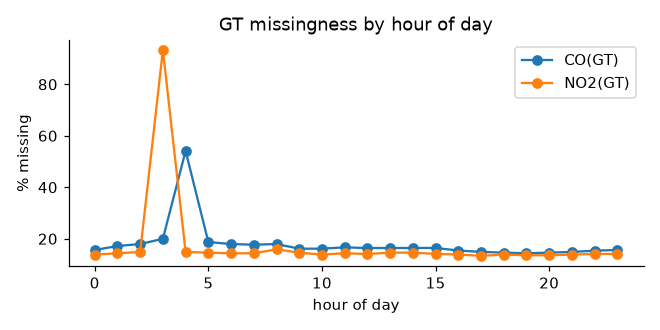
\includegraphics[width=\linewidth]{muska/missing_by_hour}
    \caption{Reference gaps by hour of day.}
    \label{fig:missing-hour}
  \end{subfigure}
  \caption{Missing data. Sensors and weather go missing together (device
  outages); the reference gases are missing far more often, mostly at night.}
  \label{fig:missing}
\end{figure}

\section{Cross-Sensitivity Study}
\label{app:cross}

\paragraph{Why raw correlation is not enough.} CO, NO$_x$ and NO$_2$ all come
from traffic and are strongly correlated with each other (Spearman
$\rho \approx 0.7$--$0.9$), so every sensor looks correlated with every gas.
A gas earned an edge to a sensor only if it explained the sensor beyond the
sensor's nominal gas, the weather and the hour.

\paragraph{Method.} For each sensor we ran forward selection over the candidate
gases on three split seeds. At each step the best candidate was kept only if
(i) adding it as a parent raised the sensor CPT's validation log-likelihood by
at least 0.02 nats per hour on average and in every seed, and (ii) its partial
Spearman correlation with the sensor, controlling for the current parents,
weather and hour, had magnitude at least 0.1 with the same sign in every seed.
We allowed at most two gas parents beyond the nominal one. The study used
$W = (T, \mathit{AH})$; the final network uses $(T, \mathit{RH})$.

\paragraph{Benzene is not an independent reference.} C$_6$H$_6$(GT) is an
almost exact cubic function of $S_2$ ($R^2 \approx 0.99998$) and is missing on
exactly the same hours. Its partial correlation with each other sensor equals
$S_2$'s own and drops to about 0.01 once $S_2$ is controlled for, so it carries
no information beyond $S_2$. We excluded it, and with it $S_2$.

\paragraph{Results.} \Cref{tab:cross} lists the kept edges and the notable
rejections. $S_4$ responds more to CO than to its nominal NO$_2$, which is why
NO$_2$ is the hardest gas to estimate. $S_5$, whose nominal O$_3$ has no
reference, behaves like a general traffic sensor. Several edges with high raw
correlation were rejected (for example $S_1 \leftarrow$ C$_6$H$_6$, raw
$\rho = 0.88$; $S_5 \leftarrow$ NO$_2$, $0.78$), because two sensors with a
common gas parent look correlated even though neither responds to the other's
gas. Some rejected edges keep a nonzero partial correlation but no reliable
likelihood gain at three bins; these are the unmodeled shared signals that can
make the posterior overconfident (\cref{sec:bn}).

\begin{table}[h]
  \centering
  \caption{Cross-sensitivity candidates (mean over three split seeds).
  $\Delta$LL: gain in validation log-likelihood per hour from adding the gas.}
  \label{tab:cross}
  \begin{tabular}{llrrl}
    \toprule
    Sensor & Gas (given) & Partial $\rho$ & $\Delta$LL (nats/h) & Decision \\
    \midrule
    $S_4$ & CO (NO$_2$)             & 0.67  & $0.157 \pm 0.022$ & kept \\
    $S_4$ & NO$_x$ (NO$_2$, CO)     & $-0.50$ & $0.033 \pm 0.002$ & kept \\
    $S_5$ & CO (none)               & 0.85  & $0.403 \pm 0.026$ & kept \\
    $S_5$ & NO$_x$ (CO)             & 0.43  & $0.052 \pm 0.014$ & kept \\
    \midrule
    $S_1$ & NO$_2$ (CO)             & 0.24  & $0.001 \pm 0.024$ & rejected \\
    $S_3$ & CO (NO$_x$)             & $-0.34$ & $0.058 \pm 0.036$ & rejected \\
    $S_3$ & NO$_2$ (NO$_x$)         & $-0.34$ & $0.018 \pm 0.024$ & rejected \\
    $S_5$ & NO$_2$ (CO, NO$_x$)     & 0.27  & $-0.012 \pm 0.003$ & rejected \\
    \bottomrule
  \end{tabular}
\end{table}

\begin{figure}[h]
  \centering
  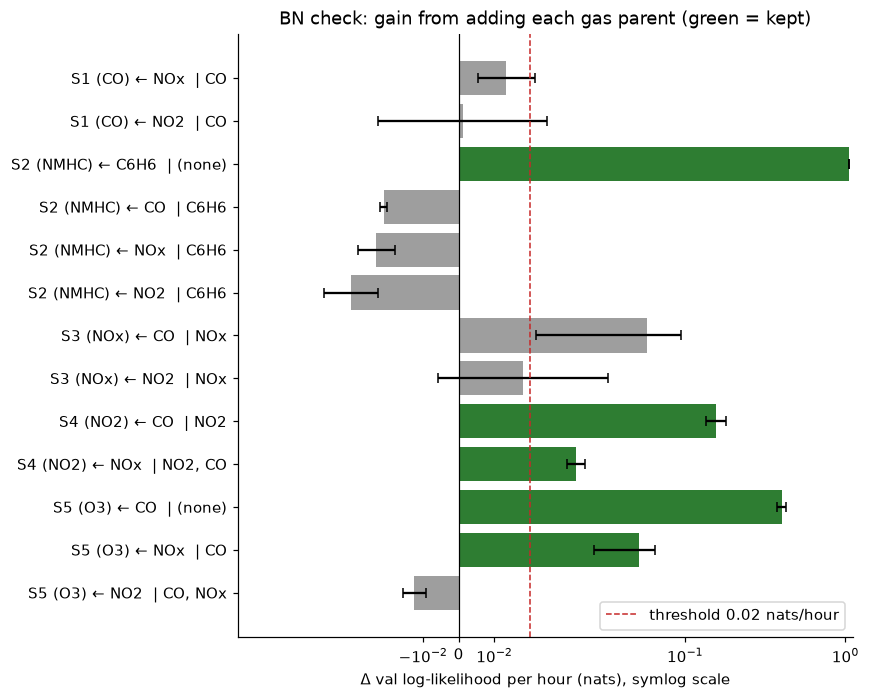
\includegraphics[width=0.7\linewidth]{studies/cross_sensitivity/bn_loglik_gain}
  \caption{Gain in validation log-likelihood from adding each candidate gas
  parent (mean $\pm$ std over three seeds; green = kept; dashed line = 0.02
  nats/h threshold).}
  \label{fig:cross-gain}
\end{figure}

\section{Code and Results}
\label{app:code}
All code and results are at \url{https://github.com/kberesfo/CSE-250A-Project}.
The final runs are the executed notebooks in \texttt{notebooks/<phase>/eval.ipynb}
and \texttt{notebooks/studies/}, which GitHub displays with their outputs;
generated tables and HTML reports are in \texttt{results/}, and figures in
\texttt{figures/}. To reproduce them, open the repository in its dev container,
download the data, and rerun every notebook on a fresh kernel:
\begin{verbatim}
uv run python scripts/get_data
make
\end{verbatim}
